\begin{comment}
\section{Architectural tactics or strategies}
	\subsection{Thread pooling: }It is used to improve scalability, by the recording handler of the Malware Application and to create multiple connections to different client phones. The Edison is connected in serial to more than one node to improve scalability( thus physical threads). The server can also handle multiple requests simultaneosly to update the database from different web clients.
	\subsection{Clustering: } All communication and events are stored on the server. This is used to improve scalability and reliability. 
	\subsection{Interception: }For any event the username and password must be visible and correct for the event to proceed. This ensures security and auditability. The website uses a Log in System, and the user may not proceed to the website if he has not logged in. The Mobile Application only works with the username and password, it is send to the Node, via NFC, in the access permission request. 
	\subsection{Authentication}The NFC module and the mobile application share a unique AID (Application Identifier) which allows only the mobile application with the correct AID to communicate with the NFC Module.
\end{comment}



\section{Quality Requirements}
\subsection{Scalability}
\begin{itemize}
\item The database on the server can handle up to 819 connections at a time. Therefor up to  819 people can simultaneously use the webpage.
\item The node is connected to the gateway via serial USB. Up to three nodes can be connected to one gateway by using a USB hub. 
\item Only one application can be installed on one phone. 
\item One user can use more than one phone. This is implemented because phones can be broken and the user could have a temporary phone, or if the user has more than one phone. The user however can only be registered for a meeting with one phone. 

\end{itemize}
%The server must be able to handle a large amount of users and users must be able to use the system simultaneously. However, the controlled access to a meeting, via the Gateway and the Node will only have a limit of one gateway per meeting and at most three nodes per meeting.

\subsection{Performance}
\begin{itemize}
\item The server uses MongoDB for its database. It has been shown that MongoDB can do more than 9000 operations per second. This is clearly a high throughput. 
\item The response time of the web page relies on the device (computer, tablet or phone) used and the speed of the Internet connection. If both the device and speed of the Internet connection are relatively high, the response time is less than 1.0 second from the server.
\item The NFC data transfer time from the phone to the node and back is less than 0.1 seconds. It appears instantly to the user. This is good for the usability, since long scanning may delay the meeting unnecessarily. 
%\item 
\end{itemize}

%The system does not have specific performance requirements, but the application to gateway operations should respond within less than 1 second, because it may delay the meeting unnecessarily. The server query operations may process up to 5 seconds long.

 \subsection{Maintainability}%The system must be easily maintainable. The application and server may be updated in time, to fit the latest technologies.
    %basically imgekeerd eweredig aan hoe lank dit jou sou vat om veranderings aan die kode te maak, goed by te sit on dit te integreer
    \begin{itemize}
        \item The code is well documented and each component has a read me file containing all the information on how the functions should be used and what it does.
        \item Unit tests have been done and are available to view as examples on how the system should be used.
    \end{itemize}

 

\subsection{Reliability}%the probability of failure-free software operation for a specified period of time in a specified environment.
\begin{itemize}
\item The server uses MongoDB for its database. MongoDB has a strict concurrent control by using locks. This means that a field may only be updated by one user at a time. This reserve the data integrity, and keep the activity log in order. 
\item Clustering is used by storing all actions and events in the database. 
\item The security keeps the data reliable.
\end{itemize}




\subsection{Availability}
\subsubsection{Application}
The application can be downloaded from the \href{https://github.com/Unsolvable-Solutions/Project-EPIC/tree/master/EPICProtectionApp/EPICAppFor4.4.2}{github link}. Ideally it would later be available on Google play store. See the user manual for installation guidelines.
\subsubsection{Web page}
The web page is available from any web browser connected to the Internet. The user simply types \url{projectepic.info} in his favourite browser.
\subsubsection{Node}
The node used is a Arduino with PN532 NFC/RFID Shield and the lights used are neopixels, it can be purchased from most electronic or robotic online stores. The source code can be downloaded from the \href{https://github.com/Unsolvable-Solutions/Project-EPIC/tree/master/EPICNode}{github link}. See the user manual for installation guidelines. 
\subsubsection{Gateway}
The gateway used is a Intel Edison board and can be purchased from most electronic or robotic online stores. The source code for the gateway can be downloaded from the \href{https://github.com/Unsolvable-Solutions/Project-EPIC/tree/master/EPICEdison}{github link}. See the user manual for installation guidelines.
\subsubsection{Server}
The server uses MongoDB and Node.js. These technologies are freely available online and are very easy to download. See the User Manual for installation guidelines.

%The application must be available from the Google play store, and the access to the web server can be found online at projectepic.info.

\subsection{Auditability}
\begin{itemize}
\item Each action performed on the server is logged in the database with a time stamp. These logs  and can be reviewed by the user that owns the meeting at any time. The logs include:
\begin{itemize}
\item A person sends a RSVP for a meeting
\item A person enters a meeting
\item A person exits a meeting
\item A user created a meeting
\item A user invited a person to the meeting
\item A person attempts to enter a meeting, but access is denied.
\end{itemize}
\item During a meeting the application keeps a log of all activities on the mobile device. The log is available for the user to view after the meeting. The log is also uploaded onto the server after the meeting. This is used so the user can see if another application attempted to turn any of the communication mechanisms on.
\item A user can view all the meetings that he owns.
\item For every event the email and password is tested. This ensures auditability in the event log. 
\end{itemize}
%The system log the entrance and exit of all meetings. For each meeting the log contains the users allowed, the users that attended, their entrance and exit times as well as the initial time and place of the meeting.

\subsection{Security}
    The system has multiple levels on which security is implemented.
\begin{itemize}
    \item Between the Node and the phone Near Field Communication (NFC) is used. NFC has its own message protocol called NDEF packaging, and for this you will need a unique ID for each sector you want to read. Plus on the higher (hardware) level you will need to get noticeable close to intercept the message packages, never-mind the strictly one-to-one structure that NFC enforces. 
    \item The Node and the Gateway communicates via a physical Serial connection (a cable). Unless the integrity of the cable is physically compromised or tampered with, the connection is secure.
    \item Between the Gateway and the server the HTTP protocol is used and this offers sufficient security for this part of the system.
    \item Then furthermore the system caters for overall security in two ways. The first is the access to the meeting room, so that not just anyone can enter the room. And secondly it stops malware (viruses) from illegally eavesdropping on your meeting.
    \item AES 128 bit encryption is used when data is send from one source to another. 
    \item The password is stored with MD5 encryption in the database. And if a user object is requested, the password hash is not included in the object. This ensures that if a hacker has breached the firewall, he still cannot get access to the password.
\end{itemize}
%The NFC components should not be hackable. 

\subsection{Monitorability}
\begin{itemize}
\item  The application constantly monitor the state of the phone. It checks if another party has tried to switch on any of the communication mechanisms. If so, the mechanism is turned of again and a notification is send to the user. This is done to prevent malware from turning on the communication mechanisms and sending any information to a hacker. 
\item When the phone is held over the node, LED lights show the current state of the processing. The LED lights have the following states.
    \begin{description}
    \item{Blue - Waiting}: The node is waiting for a phone to connect with.
    \item{Orange - Processing}: The phone has send its information to the node via NFC. The node sends the information to the gateway to check if the user has access to the meeting. And a respond is send back to the application on the phone. 
    \item{Green - Access granted}: The user may enter the meeting and the phones communication mechanisms are switched off.
    \item{Red - Access denied}: The user may not enter the meeting.
    \end{description}
\item The gateway updates the meeting information every 10 minutes, to see if the list of people attending the meeting has changed.
\item The server keeps track of the entering and exiting of meetings, this is used to report any suspicious behaviour. The reporting is done in a log on the server. The suspisious behaviour includes: 
\begin{itemize}
\item A person entering but never exiting.
\item A person entering and exiting multiple times.
\item A phones communication mechanisms being turned on during a meeting.
\end{itemize}
\end{itemize}
%The response of the Nodes is visible with the LED light showing the permission.

\subsection{Testability}
\begin{itemize}
\item Unit tests are used for each of the functions in all the components. The unit test were manual or automated. The manual testing was done where hardware was involved and where the automated test wasn't possible or applicable.
\item The integrations test have been done to combine and integrate all the separate components. %These tests were mostly manual since the end product is user dependent.
\item After the separate components have been integrated, a system test is also performed to test the flow of information and the ovarall usage of the system.
\item Usability tests are also to be performed.
\end{itemize}
%All the components must be tested separate at first, unit testing, and after completion the whole system must be tested.
%\\ For each service the pre and post conditions must be met.

\subsection{Usability}
The system is designed for the users comfort. The user simply has to open the application on his phone and hold his phone over the node to enter a room. His phone is automatically switched to protection mode. After the meeting the user simply has to hold his phone over the node again to exit the room and the protection mode is switched off again. 
\subsubsection{Application}
\begin{itemize}
\item The application has a user friendly, clean cut and intuitive interface. 
\item The application shows clear indications of what tasks could be done and what data should be typed into which fields. This is achieved by descriptive buttons, descriptive labels and clear instructions.
%\item The application can be downloaded
%\item
\end{itemize}

\subsubsection{Node}
\begin{itemize}
\item The node simply has to be plugged into the gateway and it is automatically ready to use.
\item The mobile device only has to be held over the node (less than 10 cm) for them to communicate. It is very easy to use.%, no other tricks and turns necessary.
\end{itemize}

\subsubsection{Gateway}
\begin{itemize}
\item The user do not directly use the gateway. The gateway sends data to and from the server and to and from the node. The usability of the node however is improved by the fast processing of the server.
\item The set up of the gateway for a meeting is very easy to do. The gateway is plugged into a computer and the setup menu automatically runs on the computer. The user then selects a meeting from the list of meetings and the gateway is set up. 
\end{itemize}

\subsubsection{Server}
The Server is never directly used by the user. The fast processing however do increase the usability of the gateway and the webpage.
\subsubsection{Webpage}
The website can be used by any device with a web browser.
\\The web page is made with a very simple clean cut intuitive look. There are three interfaces: The login page, the register page and the homepage. 
\\All the pages on the web page meet the following criteria to enhace the usability:
    \begin{enumerate}
    \item \textbf{Clear indications}: The pages shows clear indications of what should be done and what data should be typed into which fields. This is achieved by descriptive buttons, labels and instructions.
    \item \textbf{Simple navigation}: It is easy to go from one task to another without confusing the user. This is done to improve the performance that relies on the user.
    \item \textbf{Minimum Visual Cluttering}: Only the necessary tasks are available for the user and no extra information or pictures to distract the user. 
    \item \textbf{Simple font style}: The font colour and style is readable, this increases the usability of the web page.
    \item \textbf{Simple overall style}: This is use to create a pleasing look and not to bright or visually loud layout.
    \item \textbf{A help function}: If the user is for some reason not sure how to perform a task the help function can assist by showing the set list of tasks available and how to complete them. The help function also provides photos to make the task easier.
    \item \textbf{Fast}: The web page appear to have complete the task immediately, even though the task may still have to be completed in the background. This is however still dependent on the speed of the Internet connection that the user has.%so iets
    
    \end{enumerate}

%All the components must be intuitive and easy to use. Any user that is Android literate and computer literate must be able to use the system. The physical components must be labelled accordingly. 
%\\ The User Manual may be used for more information on any of the components. 
Note: Usability tests have not yet been done.

\subsection{Integrability}
The system consists of a mobile application, a node, a gateway, a server and a website. These different part integrate with each other to form one system. 

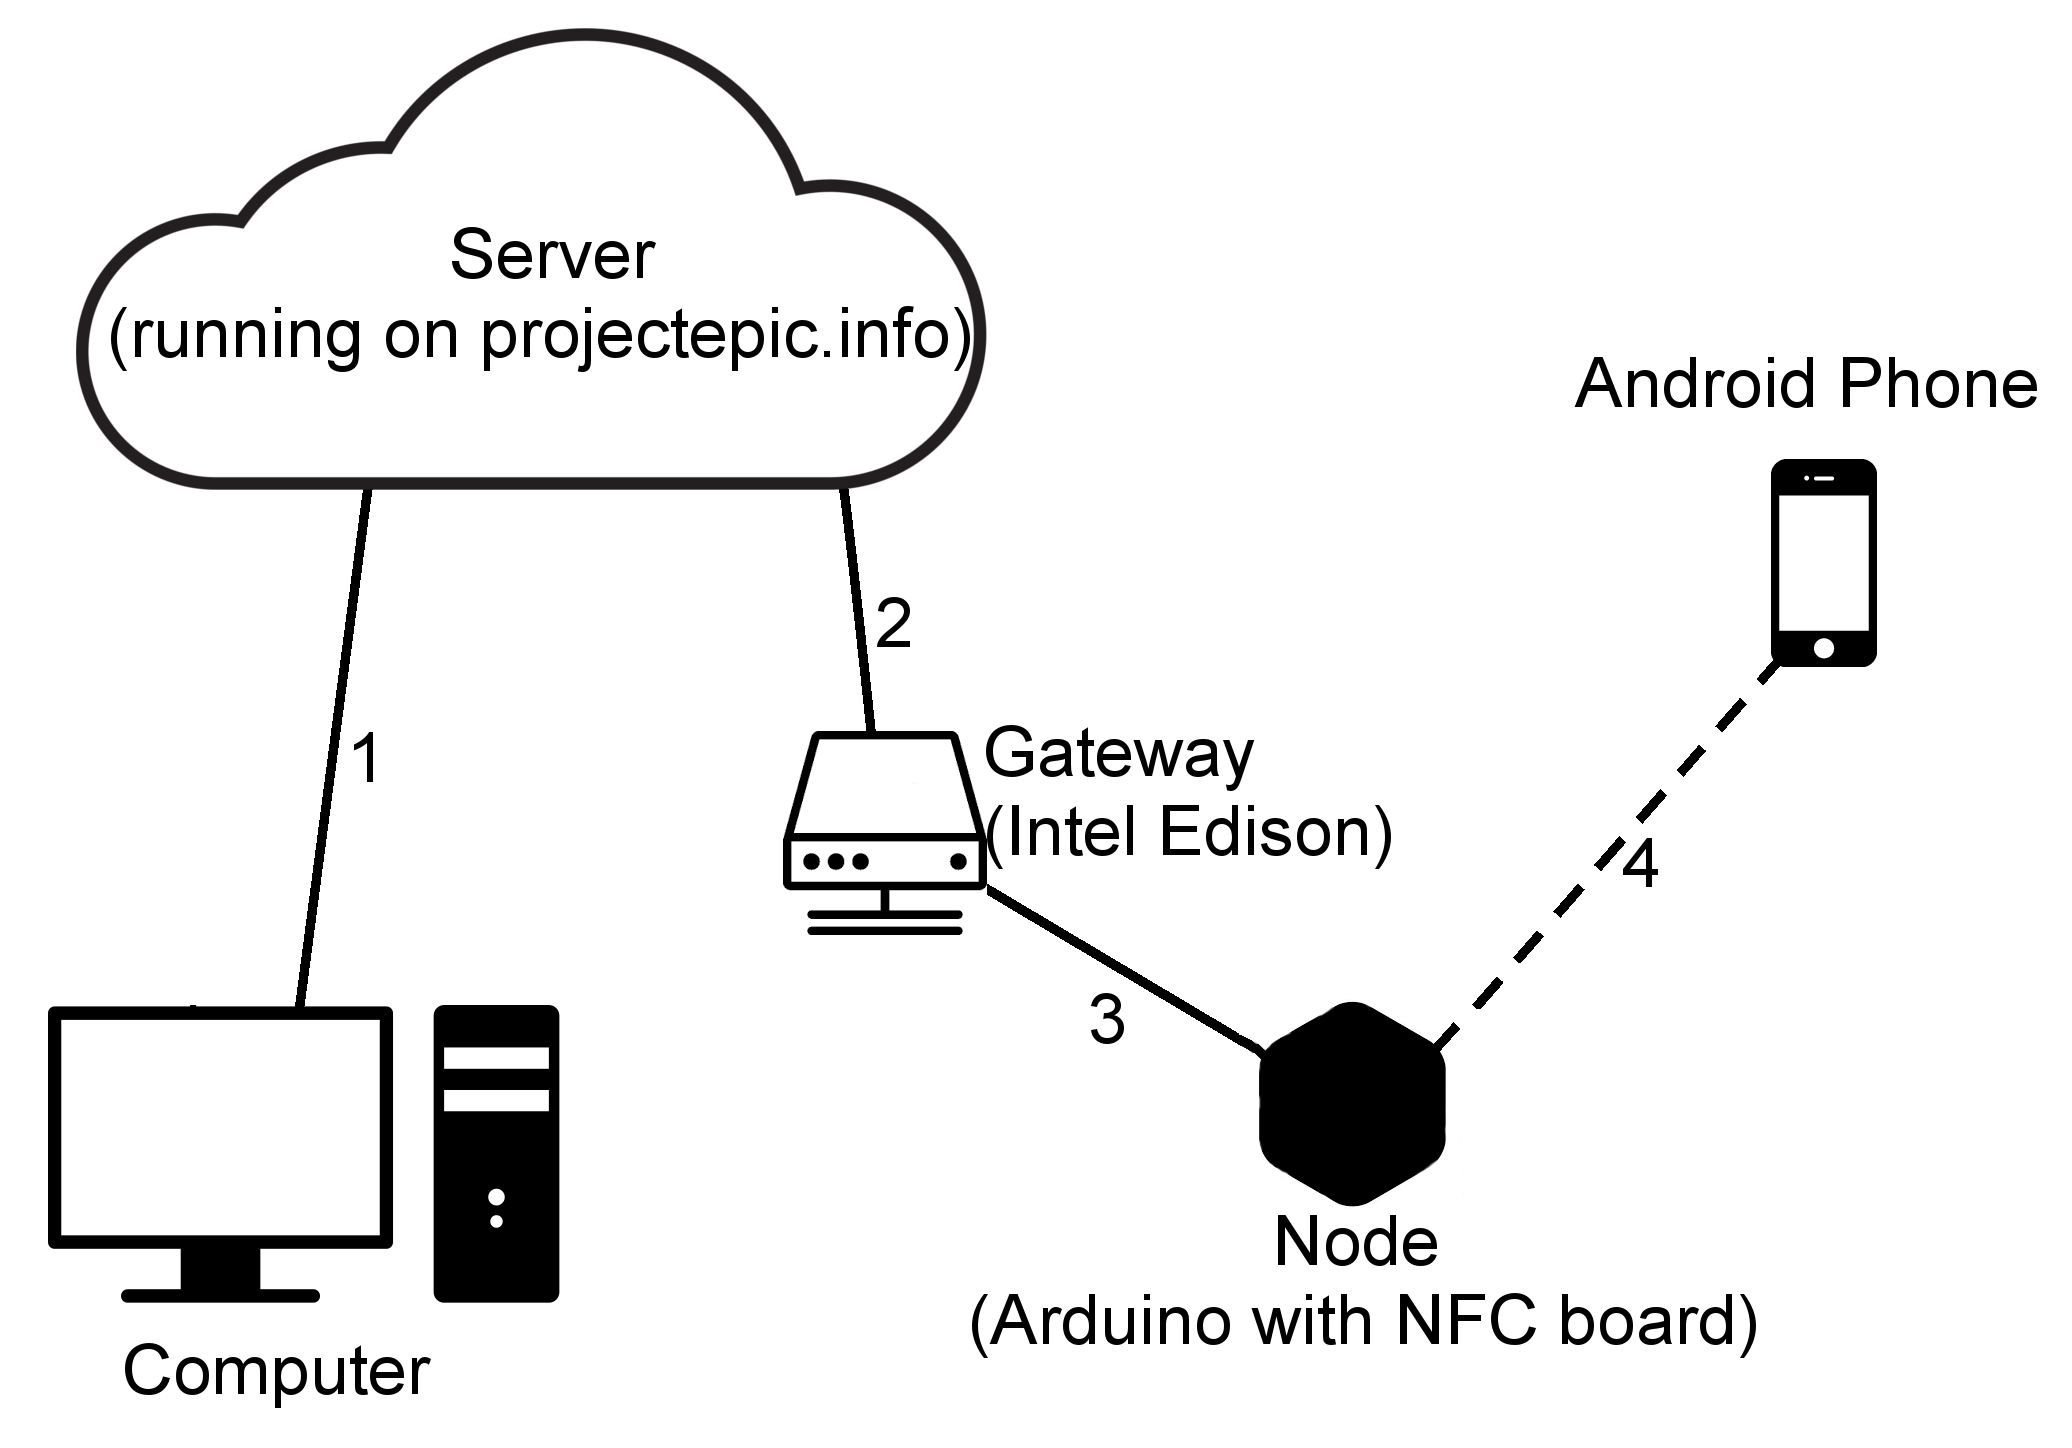
\includegraphics[width=12cm, height=8.5cm]{SystemLayout}
\begin{enumerate}
\item The website connects through the Internet via a web browser to the server. 
\item The gateway connects to the server via wifi. It relays the data from the node to the server and vice versa.
\item The gateway and node is connected using a cable. It sends the users' information, obtained from the phone via NFC, to the gateway, and transmits results  received from the gateway, via NFC to the application on the phone.
\item The phone connects to the node using NFC. The phone sends the users email address, device identification and password to the node, and the node then sends back the response from the server to the application on the phone.
\end{enumerate}

%\subsubsection{Application - Node Integration}


%The different components of the system should work together and the system must also be able to handle future additions to it.\\